\section{Experimental Data}

\textbf{Part I: Name of the Part}

\begin{table}[h]
    \centering
    \captionsetup{labelformat=empty}
    \caption{Table 14.2: Name of the Table}
    \begin{tabular}{|l|l|l|l|l|l|l|l|l|}
    \hline
        $r(cm)$ & $\theta_1$ & $\theta_2$ & $\theta_a$ & $B$ & $\theta_{corrected}$ & $\log{\theta_a}$ & $\log{\theta_{corrected}}$ & $\log{r}$ \\ \hline
        14 & 27 & 27 & 27 & 0,990 & 27,27 & 3,29 & 3,31 & 2,64 \\ \hline
        11 & 35 & 37 & 36 & 0,979 & 36,77 & 3,58 & 3,60 & 2,40 \\ \hline
        8 & 55 & 59 & 57 & 0,946 & 60,25 & 4,04 & 4,10 & 2,08 \\ \hline
        5 & 100 & 103 & 101,5 & 0,781 & 129,96 & 4,62 & 4,86 & 1,61 \\ \hline
    \end{tabular}
\end{table}


\textbf{Part II: Name of the Part}

\begin{table}[h]
    \centering
    \captionsetup{labelformat=empty}
    \caption{Table 14.5: Name of the Table}
    \begin{tabular}{|c|c|c|}
        \hline
        & Measured Value (\si{\volt}) & Calculated Value (\si{\volt}) \\
        \hline
        $V_1$ & 0.51 & 0.51 \\
        \hline
        $V_2$ & 1.66 & 1.67 \\
        \hline
        $V_3$ & 2.84 & 2.83 \\
        \hline
        $V_{12}$ & 2.17 & 2.17 \\
        \hline
        $V_{23}$ & 4.5 & 4.49 \\
        \hline
        $V_{123}$ & 5.02 & 5 \\
        \hline
    \end{tabular}
\end{table}


\begin{figure}[H]
	\centering
    \captionsetup{labelformat=empty}
    \caption{Plot 14.1: Name of the Plot}
	\pgfplotsset{width=11cm,compat=1.9}
    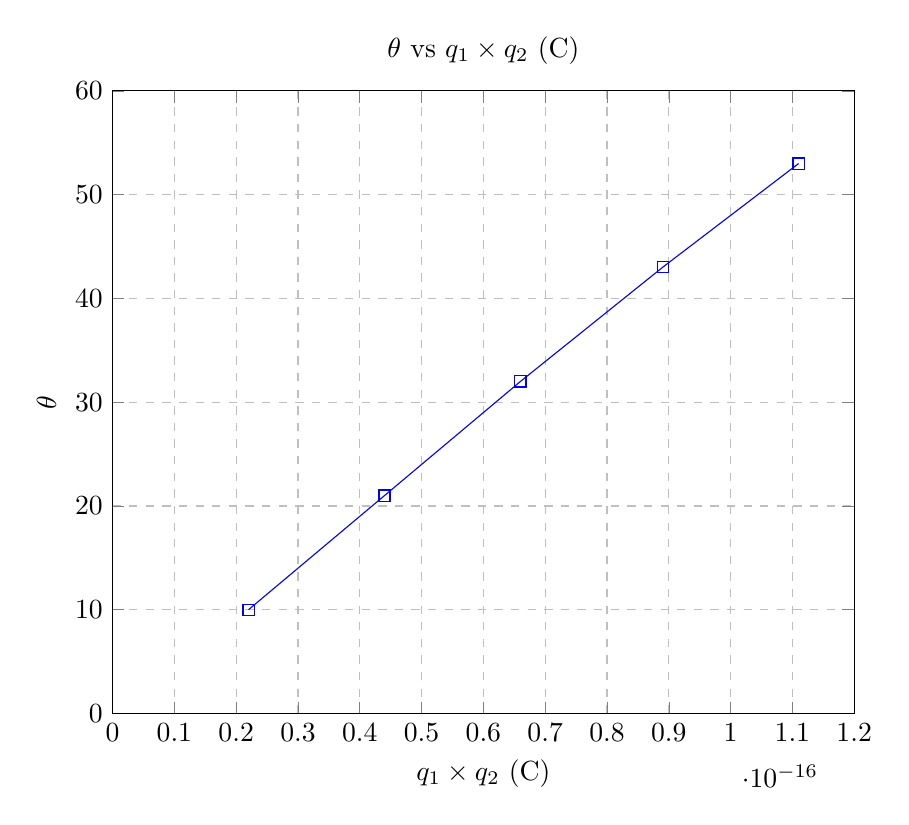
\begin{tikzpicture}
    \begin{axis}[
        title={$\theta$ vs $q_1 \times q_2$ (C)},
        xlabel={$q_1 \times q_2$ (C)},
        ylabel={$\theta$},
        xmin=0, xmax=12e-17,
        ymin=0, ymax=60,
        xtick={0, 1e-17, 2e-17, 3e-17, 4e-17, 5e-17, 6e-17, 7e-17, 8e-17, 9e-17, 10e-17, 11e-17, 12e-17},
        ytick={0, 10, 20, 30, 40, 50, 60},
        xmajorgrids=true,
        ymajorgrids=true,
        grid style=dashed,
    ]
    
    \addplot[
        color=blue,
        mark=square,
        ]
        coordinates {
        (22e-18, 10)
        (44e-18, 21) 
        (66e-18, 32)
        (89e-18, 43)
        (111e-18, 53)
        };
    \end{axis}
    \end{tikzpicture}
\end{figure}

\newpage % Starts from a new page

\textbf{Part III: Currents in Circuits}


\begin{table}[h]
    \centering
    \captionsetup{labelformat=empty}
    \caption{Table 14.6: Name of the Table}
    \begin{tabular}{|c|c|c|}
        \hline
        & Measured Value (\si{\milli\ampere}) & Calculated Value (\si{\milli\ampere}) \\
        \hline
        $I_0$ & 5 & 5.05 \\
        \hline
        $I_1$ & 5.01 & 5.05 \\
        \hline
        $I_2$ & 5 & 5.05 \\
        \hline
        $I_3$ & 5 & 5.05 \\
        \hline
    \end{tabular}
\end{table}

\begin{table}[h]
    \centering
    \captionsetup{labelformat=empty}
    \caption{Table 14.7: Name of the Table}
    \begin{tabular}{|c|c|c|}
        \hline
        & Measured Value (\si{\milli\ampere}) & Calculated Value (\si{\milli\ampere}) \\
        \hline
        $I_0$ & 69.7 & 74.08 \\
        \hline
        $I_1$ & 47.5 & 50 \\
        \hline
        $I_2$ & 15 & 15.15 \\
        \hline
        $I_3$ & 8.7 & 8.93 \\
        \hline
        $I_4$ & 69.7 & 74.08 \\
        \hline
    \end{tabular}
\end{table}

\FloatBarrier % creates a barrier that prevents any floats
